% A simple LaTeX template for lab reports in TDT4258 Energy Efficient Computer Design
% by Yaman Umuroglu (yamanu@idi.ntnu.no)
% Feel free to customize the style as you see fit, but the chapters/sections mentioned in the
% template should be included with the appropriate content.

\documentclass[abstract=on,a4paper]{scrreprt}
\usepackage[utf8]{inputenc}


\usepackage{natbib}
\usepackage{graphicx}
\usepackage{tikz}
\usepackage{pgfplots}
\pgfplotsset{compat=1.12}
\usepackage{textcomp}

%The packages that I added to the template
\usepackage{float}
\usepackage{indentfirst}
\usepackage{listings}
\usepackage{xcolor}
\usepackage{lipsum}
\usepackage{array}
\usepackage{multirow}
\usepackage{caption}
\usepackage{hyperref}

\hypersetup{%
  colorlinks=false,% hyperlinks will be black
  linkbordercolor=red,% hyperlink borders will be red
  linkcolor=blue
  pdfborderstyle={/S/U/W 1}% border style will be underline of width 1pt
}

\definecolor{codegreen}{rgb}{0,0.6,0}
\definecolor{codegray}{rgb}{0.5,0.5,0.5}
\definecolor{codepurple}{rgb}{0.58,0,0.82}
\definecolor{backcolour}{rgb}{0.95,0.95,0.92}


\lstdefinestyle{mystyle}{
    backgroundcolor=\color{backcolour},
    commentstyle=\color{codegreen},
    keywordstyle=\color{magenta},
    numberstyle=\tiny\color{codegray},
    stringstyle=\color{codepurple},
    basicstyle=\ttfamily\footnotesize,
    breakatwhitespace=false,
    breaklines=true,
    captionpos=b,
    keepspaces=true,
    numbers=left,
    numbersep=5pt,
    showspaces=false,
    showstringspaces=false,
    showtabs=false,
    tabsize=4
}

\newcommand\MyBox[2]{
  \fbox{\lower0.75cm
    \vbox to 1.7cm{\vfil
      \hbox to 1.7cm{\hfil\parbox{1.4cm}{#1\\#2}\hfil}
      \vfil}%
  }%
}

\lstset{style=mystyle}

% Edit the meta.tex file to change title, group number and author names
% Fill in the report title, group number and student names here
\newcommand{\mytitle}{Sudoku Digit Recognition and Classification}
\newcommand{\myauthor}{Deniz Gokcin}

\title{\mytitle}
\author{\myauthor}
\date{\today}



\begin{document}
% The title page, edit if you want to customize it
\begin{titlepage}
\centering

\includegraphics[height=3.5cm]{images/ozu.jpg}\\[1cm]   
\begin{center}

% Upper part of the page
~\\[1.5cm]

\textsc{\Large CS523 Computer Vision\\Report}\\[0.5cm]

% Set the title of the Document between two horizontal lines
\hrule ~\\[0.2cm]
{\huge \bfseries \mytitle}\\[0.4cm]		% print the title of the document
\hrule ~\\[1.5cm]

% Additional Information about the document
\begin{minipage}{0.4\textwidth}
    \centering
	\large
		%\emph{Group \mygroupnumber:}\\~\\
		\myauthor
\end{minipage}

\vfill

% Bottom of the page
{\large \today}

\end{center}
\end{titlepage}



% Main matter - edit corresponding file under content/ to change
\section*{Introduction}

This report explains the implementation details of CS523 Computer Vision
Assignment 2, which is about training a kNN classifier on the MNIST dataset,
reducing the dimensions with Principal Component Analysis(PCA) and using the
classifier on the Sudoku Dataset to recognize the digits. I will explain the
idea behind PCA for reducing the dimensions, the kNN classifier, processing
methods I have used to extract digits from the Sudoku Dataset and lastly comment
on my results.

To run the code, there needs to be an images directory where the .dat files and
.jpg files are located. Also
\href{https://pypi.org/project/python-mnist/} {python-mnist} needs to be
installed to load the MNIST dataset into numpy arrays.


\section*{About Principal Component Analysis} Principal Component Analysis(PCA)
is an algorithm used for dimensionality reduction. In the MNIST hand written
digits dataset, each image comes as vectors of dimension 784. However, we do
not need all the dimensions contain classifying an image.  The idea is,
compressing a matrix with a lot of features into a smaller matrix, with less
features which preserves as much of the information in the full matrix as
possible.

In my PCA algorithm, I first did stuff.
\begin{figure}[H]
    \centering
    \includegraphics[width=\textwidth]{images/before-after-pca.png}
    \caption*{PCA results}
    \setlength{\belowcaptionskip}{-20pt}
    \setlength{\abovecaptionskip}{-20pt}
\end{figure}


\begin{figure}[H]
    \centering
    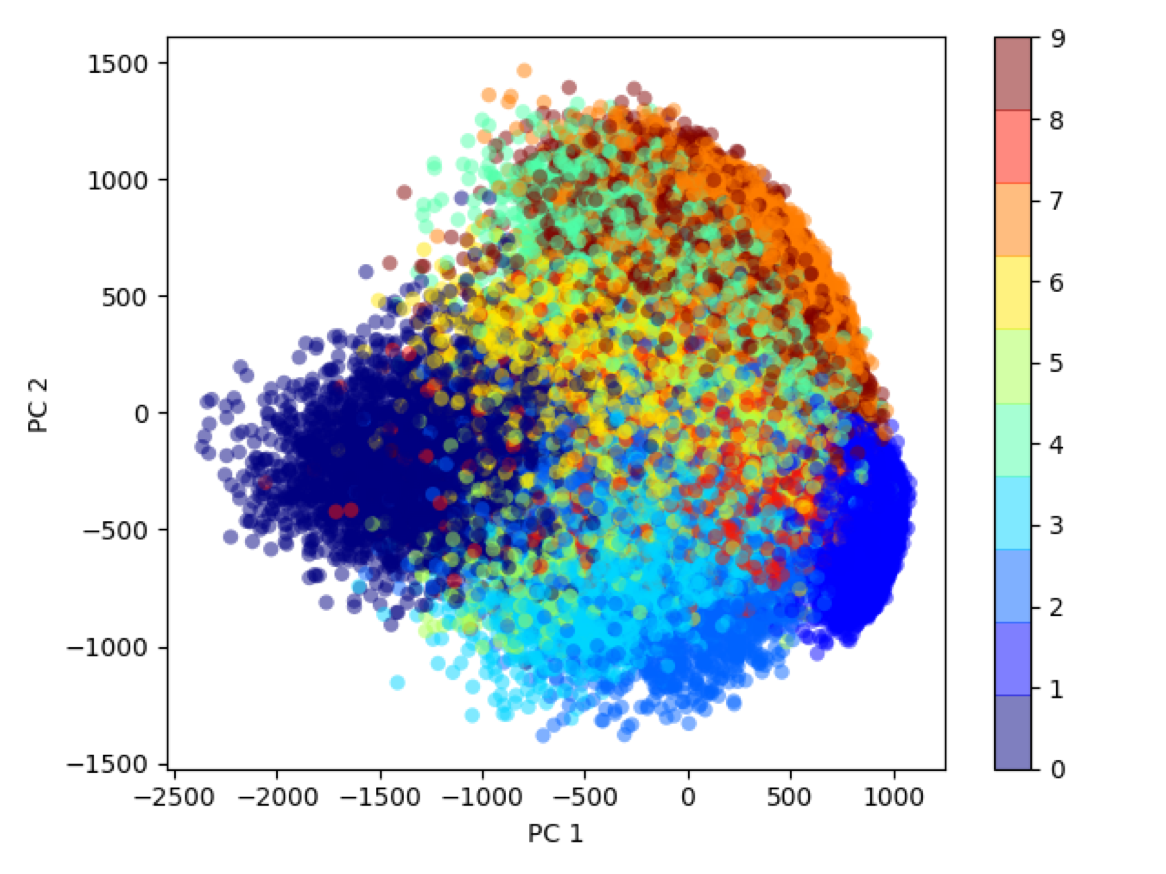
\includegraphics[width=\textwidth]{images/pca.png}
    \caption*{PCA results}
    \setlength{\belowcaptionskip}{-20pt}
    \setlength{\abovecaptionskip}{-20pt}
\end{figure}


\section*{About k-Nearest Neighbor Algorithm}

\lipsum[1-1]

\begin{figure}[H]
    \centering
    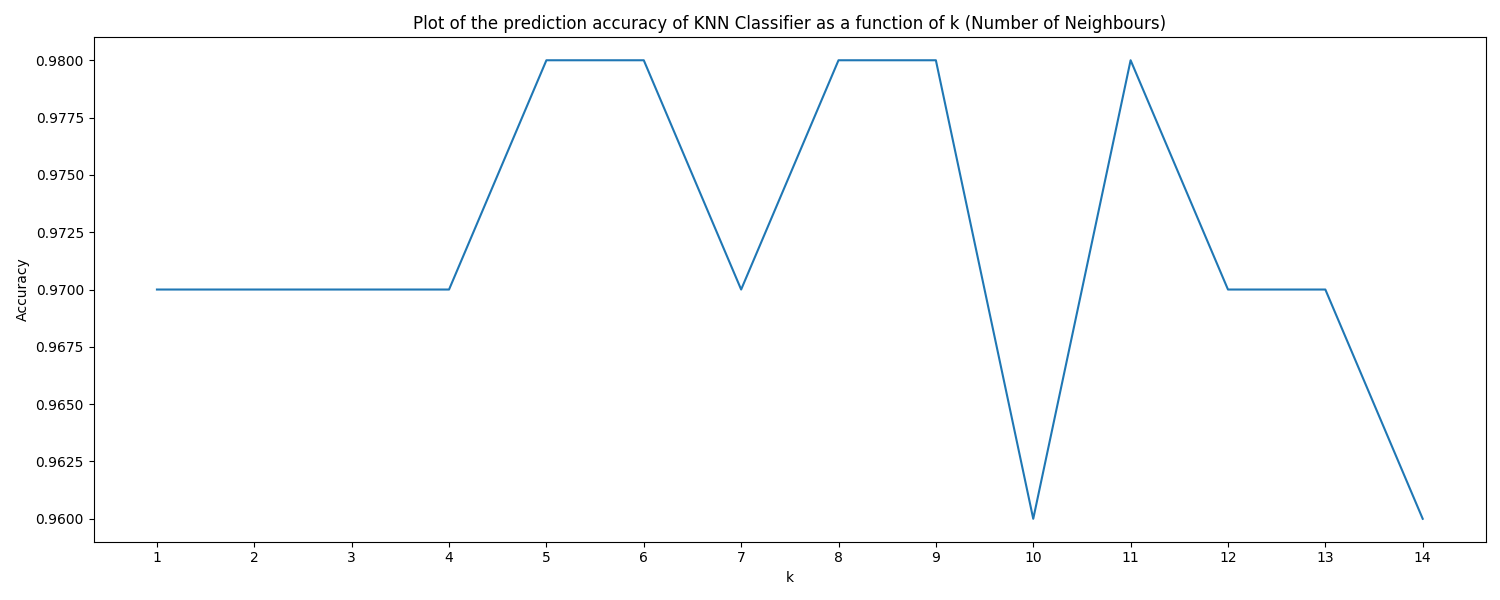
\includegraphics[width=\textwidth]{images/knn.png}
    \caption*{Prediction accuracy of kNN Classifier \\
    as a function of k (Number of Neighbours)}
    \setlength{\belowcaptionskip}{-20pt}
    \setlength{\abovecaptionskip}{-20pt}
\end{figure}


%\lipsum[1-1]

\begin{table}[H]
    \centering
    \begin{tabular}{llllllllllll}
        Predicted & 0 & 1     & 2     & 3     & 4    & 5    & 6    & 7     & 8    & 9    & All \\
        Actual &      &       &       &       &      &      &      &       &      &      &        \\
        0      &  975 &     1 &     1 &     0 &    0 &    1 &    1 &     1 &    0 &    0 &    980 \\
        1      &    0 &  1131 &     1 &     0 &    0 &    0 &    3 &     0 &    0 &    0 &   1135 \\
        2      &    7 &     1 &  1003 &     0 &    1 &    0 &    3 &    11 &    6 &    0 &   1032 \\
        3      &    0 &     2 &     4 &   973 &    0 &   13 &    0 &     6 &   10 &    2 &   1010 \\
        4      &    0 &     0 &     0 &     0 &  960 &    0 &    4 &     2 &    0 &   16 &    982 \\
        5      &    3 &     2 &     1 &     9 &    1 &  868 &    5 &     1 &    1 &    1 &    892 \\
        6      &    4 &     4 &     0 &     0 &    3 &    0 &  947 &     0 &    0 &    0 &    958 \\
        7      &    1 &    20 &    10 &     0 &    2 &    0 &    0 &   985 &    0 &   10 &   1028 \\
        8      &    3 &     0 &     3 &    14 &    4 &    5 &    1 &     2 &  938 &    4 &    974 \\
        9      &    4 &     3 &     3 &    10 &   14 &    6 &    1 &     7 &    4 &  957 &   1009 \\
        All    &  997 &  1164 &  1026 &  1006 &  985 &  893 &  965 &  1015 &  959 &  990 &  10000 \\
    \end{tabular}
    \caption*{Confusion Matrix of kNN classifier with 6 neighbors\\
    Accuracy: 97.37\%}
\end{table}

%\cite{watson_2020s}

%\begin{lstlisting}[language=Python, caption=Caption for the snippet]
%# Code snippet
%print("I am a code snippet!")
%\end{lstlisting}

%\newpage

\section*{Results}

\lipsum[1-3]

\section*{Section Title}
\lipsum[1-2]



% Bibliography - edit references.bib and use the \cite command in text
%\bibliographystyle{plain}
%\bibliography{references}

\end{document}

